% mnm-implosion-problem.tex

\section{MNM implosion problem}
\label{mnm-implosion-sec}
%
This example shows the use of the Python functions to set up
a very simple flow geometry with a reasonably complex initial flow state 
and then to test the symmetry of the computed flow solution.
This test was suggested by Dr. Michael Macrossan.
The flow field should be axisymmetric but it is computed on a square grid,
so any grid-aligned flux calculation problems should be highlighted.
Run the case with the following commands:\\
%
\topbar\\
\texttt{\$ cd $\sim$/cfcfd2/examples/eilmer3/2D/implosion/}\\
\texttt{\$ ./imp\_run.sh}\\
\bottombar\\
%
and, within a couple of minutes, you should end up with a number of files
with various solution data plotted.
Figure\,\ref{implosion-initial-density-fig} shows the initial density field
in a quiescent gas.
This field is approximately axisymmetric and is initialized by computing an estimate
for fraction of each cell inside the nominal radius of 1.0 and then weighting the
density value by that fraction.
The code for this calculation dominates the imput script in Section\,\ref{implosion-py-file}

\begin{figure}[htbp]
\begin{center}
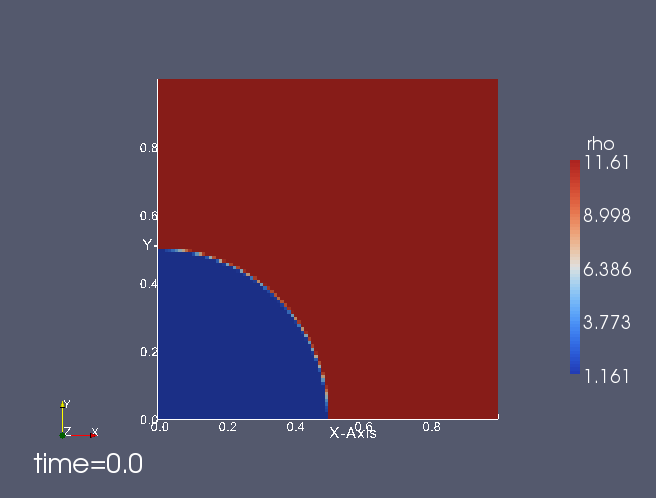
\includegraphics[width=10cm]{../2D/implosion/density-t0000.png}
\end{center}
\caption{Initial density field for the implosion problem.}
\label{implosion-initial-density-fig}
\end{figure}

\medskip
Figure\,\ref{implosion-final-density-fig} shows the density field at the end of
time-stepping, when $t=0.296 ~ \frac{L}{a}$ where $a$ is the initial sound speed of the gas
and L is a nominal length scale.
At this time the shock has propagated into the origin, reflected and passed back out 
through the contact surface.
Symmetry of the solution is not perfect but it is pretty good.
Figure\,\ref{implosion-density-profiles-fig} shows the density profiles for a number of radial slices.


\begin{figure}[htbp]
\begin{center}
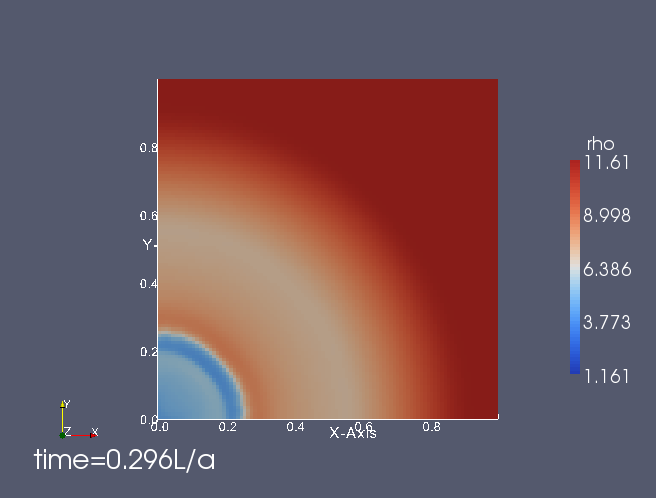
\includegraphics[width=10cm]{../2D/implosion/density-t9999.png}
\end{center}
\caption{Final density field for the implosion problem.}
\label{implosion-final-density-fig}
\end{figure}

\begin{figure}[htbp]
\begin{center}
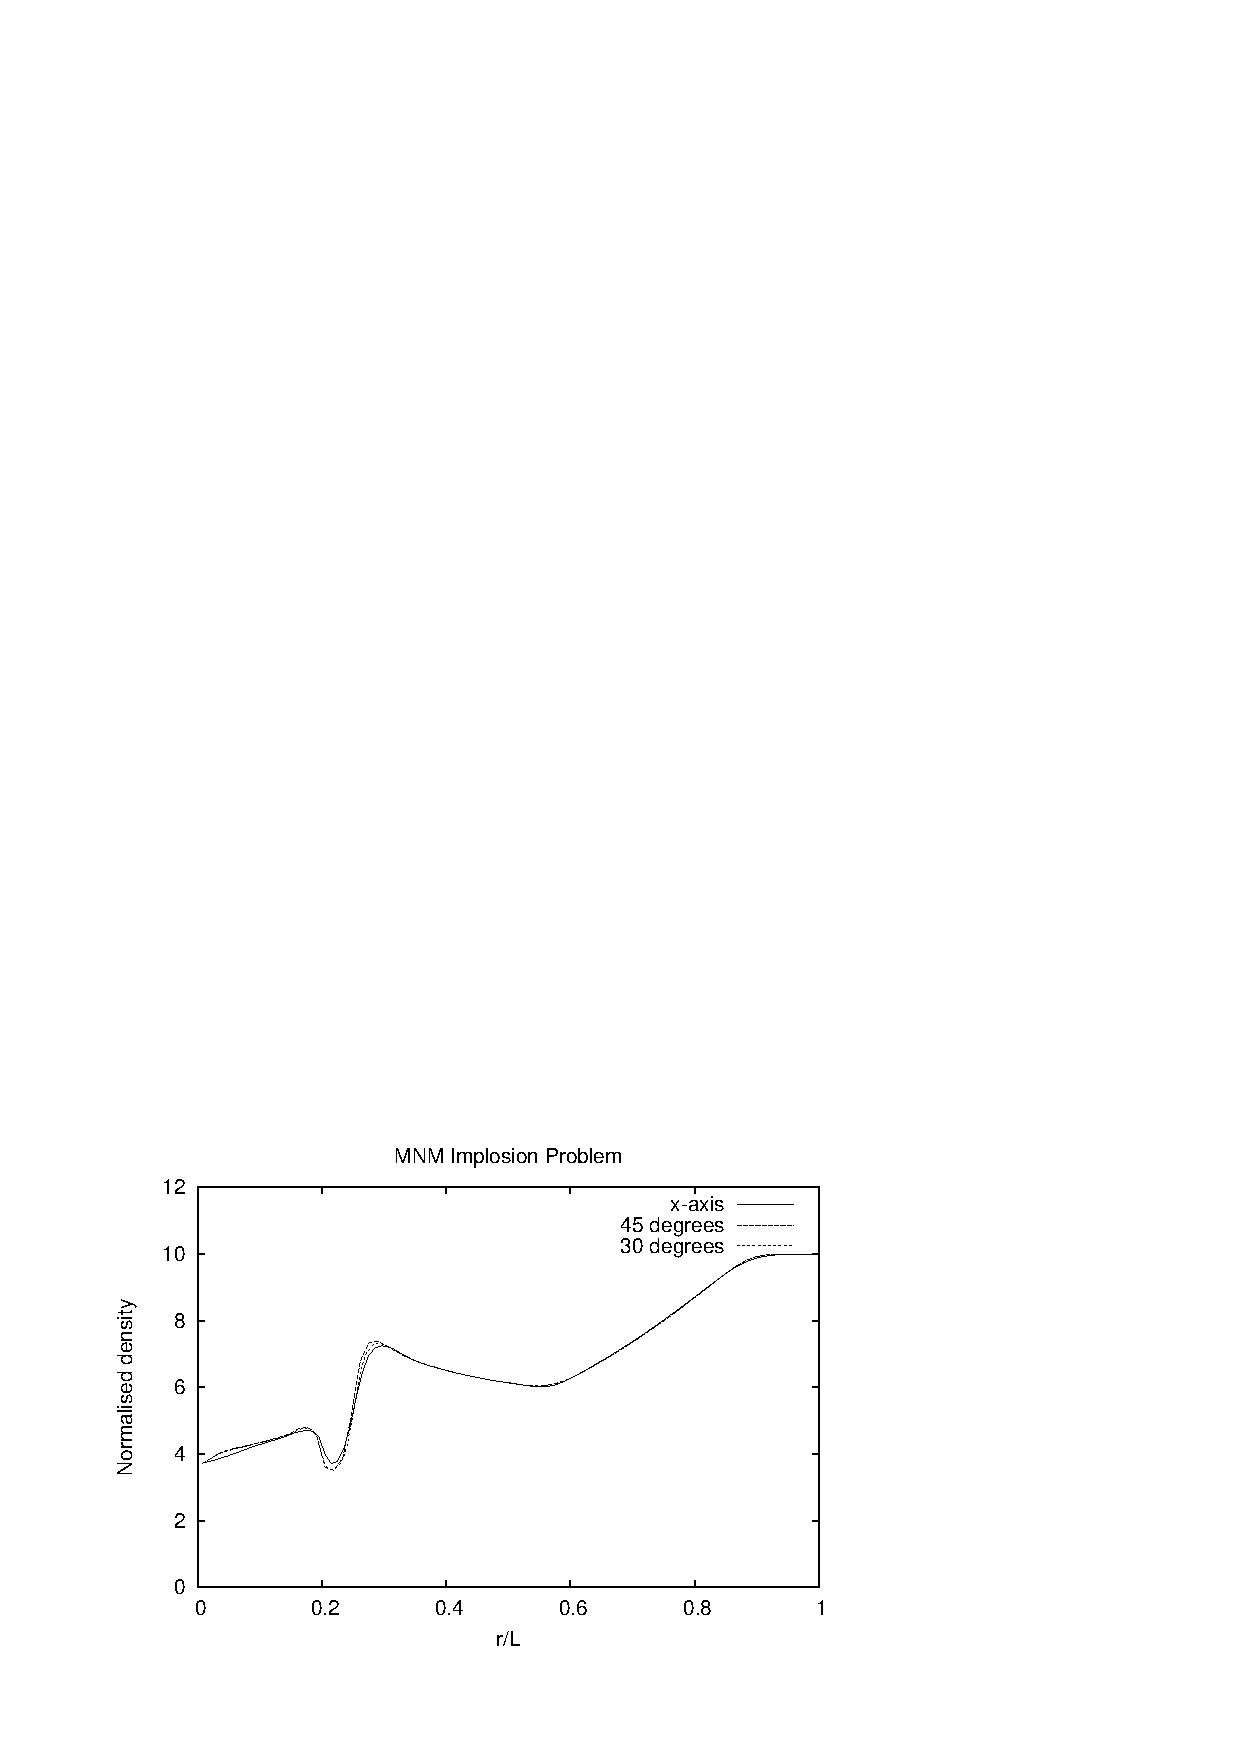
\includegraphics[width=10cm,viewport=55 49 397 293,clip=true]{../2D/implosion/density-vs-radius.pdf}
\end{center}
\caption{Density profiles at the final time for the implosion problem.}
\label{implosion-density-profiles-fig}
\end{figure}

\medskip

\newpage

\subsection{Input script (.py)}\index{geometric element!PyFunctionSurface!example of use}
\index{gas model!change\_ideal\_gas\_attribute!example of use}
\label{implosion-py-file}
\topbar
\lstinputlisting[language={}]{../2D/implosion/imp.py}
\bottombar


\subsection{Shell scripts}
\label{implosion-sh-files}
\topbar
\lstinputlisting[language={}]{../2D/implosion/imp_run.sh}
\bottombar

\subsection{Notes}
\begin{itemize}
\item This example shows how to change an attribute of the ideal gas model,
  specifically, the ratio of specific heats.
  Look for the call to the function \texttt{change\_ideal\_gas\_attribute}
  in the input script. 
\item It also shows off the \texttt{--slice-along-line} option for 
  the postprocessor \texttt{e3post.py}.
\end{itemize}
